\section{Results}
\label{results}

This section is divided into two parts. In the first, we evaluate the machine learning algorithm and its results for anomaly detection by Intrusion detection system. In the second, we
focus on the overall NADIR system by using Snort to run an experiment in which network attacks are detected and response to with forged honey-service information. NADIR uses the J48 decision tree based learning algorithm to create Snort rules on the fly in response to previously observed network features. An example of a subsection of a classification tree is provided in Figure \ref{fig:J48tree}. Table \ref{table:J48result} and Figure \ref{fig:sum-roc} show the accuracy results of the J48 algorithm and ROC curve for each type of traffic.

\begin{table*}
\begin{center}
\begin{tabular}[width=\textwidth]{llllllllll}
\multicolumn{10}{l}{\bfseries === Detailed Accuracy By Class ===}\\
\\
 & TP Rate & FP Rate & Precision & Recall & F-Measure & MCC & ROC Area & PRC Area & Class\\
 & 0.996 & 0.033 & 0.994 & 0.996 & 0.995 & 0.967 & 0.987 & 0.995 & NORMAL\\
 & 0.976 & 0.003 & 0.981 & 0.976 & 0.979 & 0.975 & 0.991 & 0.977 & Probe\\
 & 0.820 & 0.001 & 0.890 & 0.820 & 0.854 & 0.853 & 0.957 & 0.777 & R2L\\
 & 0.934 & 0.000 & 0.959 & 0.934 & 0.947 & 0.946 & 0.980 & 0.950 & DoS\\
 Weighted Avg. & 0.991 & 0.029 & 0.991 & 0.991 & 0.991 & 0.967 & 0.987 & 0.990 & \\
\end{tabular}
\end{center}
\caption{Accuracy Result of J48 algorithm (based on our dataset)}
\label{table:J48result}
\end{table*}

\begin{figure}[h!]
	\centering
	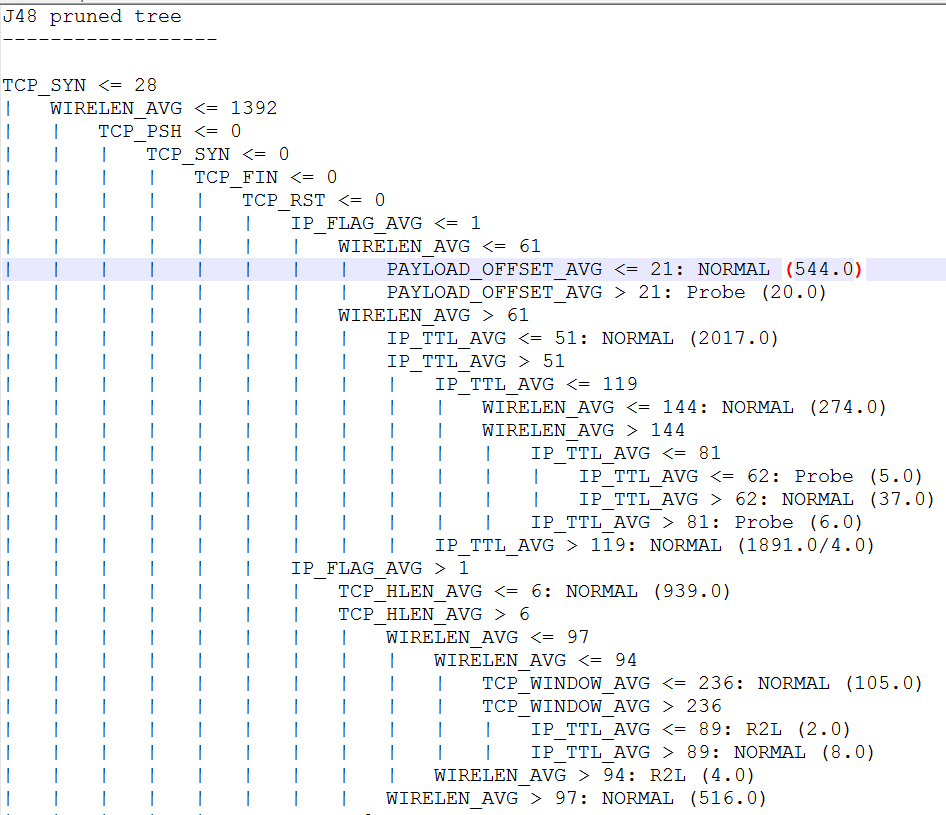
\includegraphics[width=\linewidth]{J48_tree.png}
	\caption{Sub part of pruned tree J48 Decision (based on our dataset)}
	\label{fig:J48tree}
\end{figure}

\begin{figure*}
	\centering
	\begin{subfigure}[t]{0.4\textwidth}
            \centering
            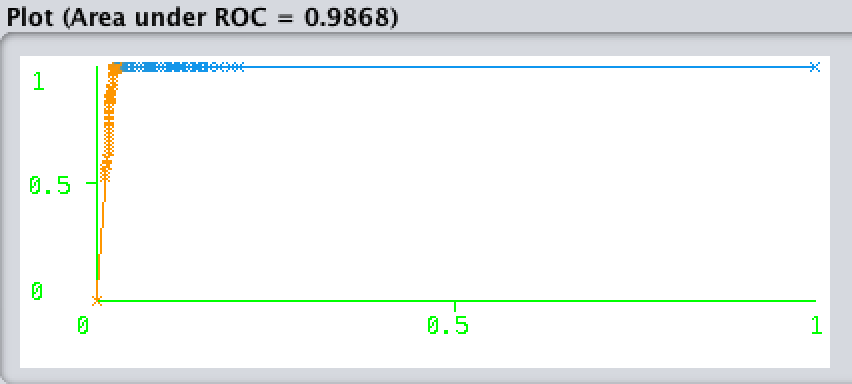
\includegraphics[width=\textwidth]{NORMAL.png}
            \caption{ROC-NORMAL}
            \label{fig:normal-roc}
        \end{subfigure}
        \quad
        \begin{subfigure}[t]{0.4\textwidth}
            \centering
            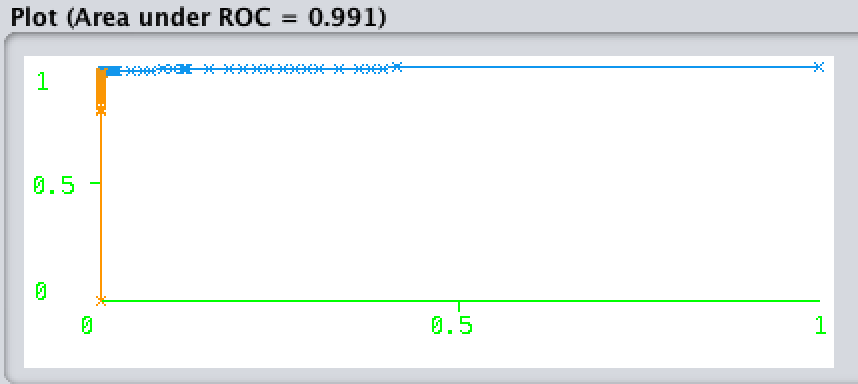
\includegraphics[width=\textwidth]{ProbeAttack.png}
            \caption {ROC-Probe}
            \label{fig:probe-roc}
        \end{subfigure}
        \vskip\baselineskip
        \begin{subfigure}[t]{0.4\textwidth}
            \centering
            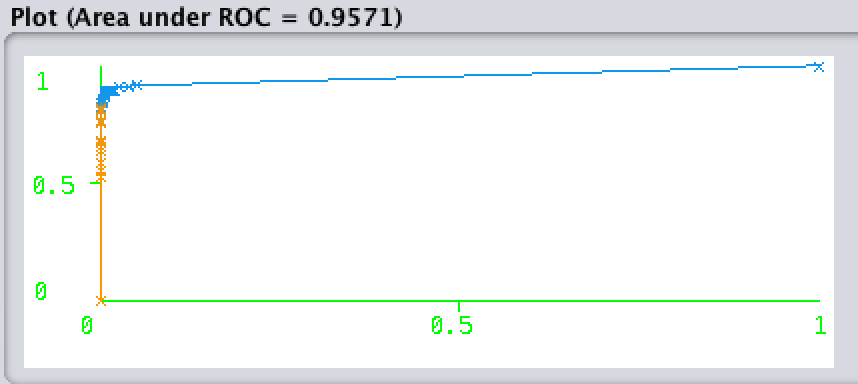
\includegraphics[width=\textwidth]{R2L.png}
            \caption{ROC-R2L}
            \label{fig:r2l-roc}
        \end{subfigure}
        \quad
        \begin{subfigure}[t]{0.4\textwidth}
            \centering
            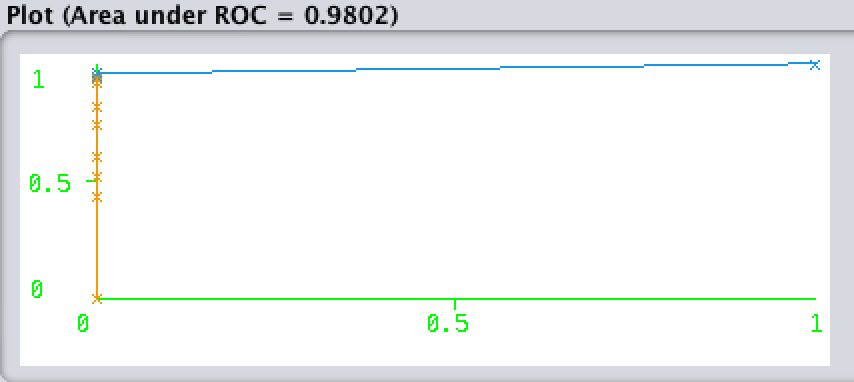
\includegraphics[width=\textwidth]{DoS.png}
            \caption{ROC-DoS}
            \label{fig:dos-roc}
        \end{subfigure}
        \caption{The ROC Curves for each type of traffic}
        \label{fig:sum-roc}
\end{figure*}

We evaluated the end-to-end NADIR system which collects network features, uses them to generate Snort rules, and then pushes them into the configuration of an existing Snort service, which is then 
restarted. This results in an overall system which uses the J48 machine learning algorithm to detect network anomalies. In response, it generates Snort rules dynamically and replaces  them without 
incurring any lost packets. If NADIR detects any attempt to attack the machine, it can respond by taking action such as dropping incoming packets coming from the suspected attacker's IP address.

%We use a common rule for DOS and DDOS detection so machine can detect both of them.

We tested the complete NADIR system by launching attacks against a computer with it installed at known times to provide ground truth. We then calculated area under the ROC curve (AUC) values to evaluate 
the tradeoff between true positive (TP) and false positive (FP) rates of our system. The AUC for detecting these attacks was 0.987 for Normal traffic. NADIR classified Probe, R2L, DoS attacks with AUC 
values of 0.991, 0.950, and 0.980 respectively. Although some errors of both types were made by NADIR's classifier, rates were low; for example, the prediction results of DoS attacks show a 0\% false 
positive rate.
